\begin{titlepage}
\begin{center}
    \large Mitschrift zur Vorlesung
    
    \vspace{10pt}
    
    \huge Mathematische Methoden \\
    \huge der Physik II
    
    \vspace{10pt}
    
    \large Oliver Benz
    
    \vspace{60pt}

    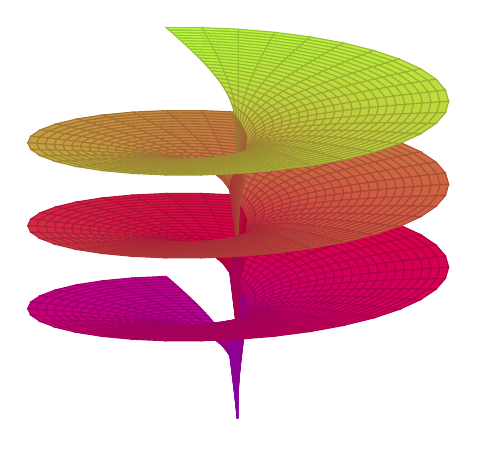
\begin{tikzpicture}
        \begin{axis}[trig format plots=rad,view={70}{18},
            colormap={adopted}{rgb255(0cm)=(151,0,250);
            rgb255(1cm)=(219,0,70);rgb255(2cm)=(186,255,60)},
            z buffer=sort,zmin=-3.5*pi,
            hide axis
            %,colormap/cool
            ]
        
        \addplot3
            [surf,domain=0.001:4,domain y=-3*pi:3*pi,samples=25,samples y=109]
            ({x*cos(y)},{x*sin(y)},{ln(x)+y});
        \end{axis}
    \end{tikzpicture}
    
    \vspace{60pt}
    
    \large Universität Innsbruck
    
    \large Wintersemester 2021
    
\end{center}
\end{titlepage}